\subsection{Thermal Control System (THC)}

Due to the ever longer mission times and larger amounts of energy used by CubeSats,
the thermal control system is gaining in importance. Each component of a CubeSat
has an operational and survival range of temperatures that are attempted by a
miniaturized thermal management system to maintain. \cite{MIST_cubesat}

The objective of TCS is to monitor and regulate the temperature within the satellite.
If the temperature leaves the viable range of a particular component,
system-critical failures may occur.

\subsubsection{Heat transfer}


The usual ways of heat transfer are conduction, convection and radiation. In the
case of CubeSat, convection is lost due to the vacuum. In the interior of CubeSats,
heat transfer is dominated by conduction due to the small temperature differences
of the components. However, external radiation has a much greater influence on
the overall heat balance.

This can be manipulated by the radiative properties, such as solar absorptivity
($\alpha$) and infrared (IR) emissivity ($\epsilon$). Solar absorptivity governs
how much of the impinging solar flux a spacecraft absorbs, while IR emissivity
determines how well a spacecraft emits its thermal energy to space, relative to
a perfect blackbody emitter. These properties are almost entirely surface
properties of a material, and can be modified simply by adding specialized
coatings, platings, polishings, or even adhesive tapes of specific materials.

\begin{figure}[h]
	\centering
	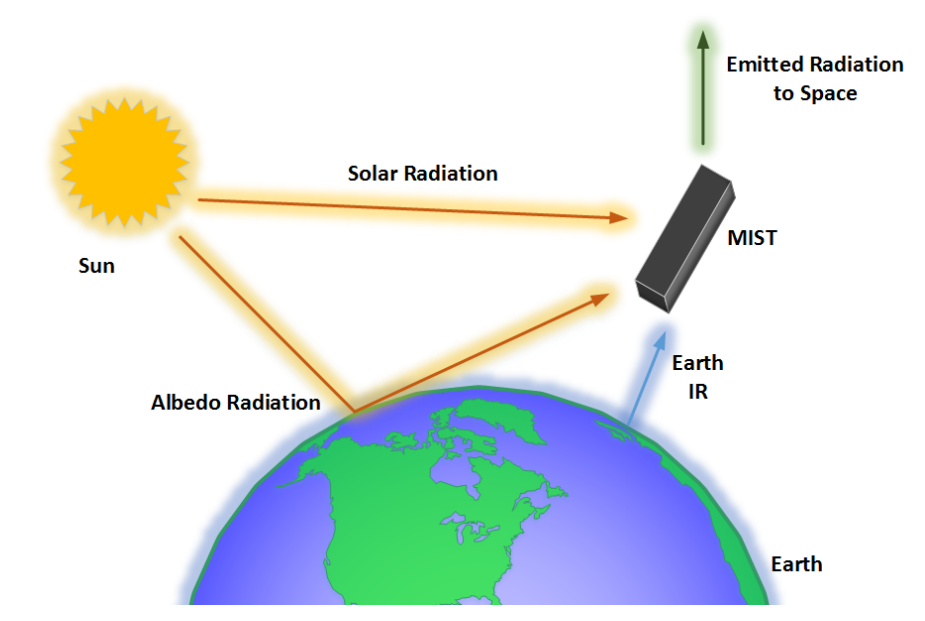
\includegraphics[width=0.8\textwidth]{img/radiation_space.png}
	\caption{Radiation sources in orbit around Earth}
	\label{fig:radiation_space}
\end{figure}

\subsubsection{Thermals Control Systems}

\paragraph{Active Thermal Control Systems}

Active TCSs require a supply of electrical energy. For example, electrical resistance
heater or the use of cryogenic materials. The great challenge of keeping energy
consumption of CubeSats small limits the use of active thermal controls systems.
Exceptions are made for particularly sensitive devices such as batteries, cameras
and certain electronic components. Active thermal control systems are much more
efficient than passive ones, but do not play a relevant role in this project.
The only exception will be a resistance heater, which will keep the battery in
the temperature surviving range during the launch and before the CubeSat is put
into operation. This safety measure represents a backup during the mission and is
monitored by temperature sensors on the battery and the control unit. In this
way the power supply can be guaranteed in the event of an emergency situation.

\begin{table}[h!]
	\centering
	\begin{tabular}{c c c}
		\hline
		\textbf{Products} & \textbf{Manufacturer} & \textbf{TRL Status} \\
		\hline
		Electrical Heaters & \pbox{8cm}{Minco Products, Inc. and\\
		All Flex Flexible Circuits, LLC.} & 9 \\ \hline
		Mini Cryocoolers & \pbox{8cm}{Ricor-USA, Inc., Creare Sunpower Inc.,\\Nortrop Grumman, NASA Jet Propulsion Laboratory\\	Lockheed Martin Space Systems Company} & 6 \\ \hline
		\pbox{8cm}{Flexible and enhanced \\Active Thermal Straps\\(FEATS)} & LoadPath & 6 \\ \hline
	\end{tabular}
	\caption[State-of-art active thermal control systems]{State-of-art active thermal control systems \cite{NASA_thermal}}
	\label{tab:active_thermal}
\end{table}

\paragraph{Pasive thermal control systems}

A passive TCS does not consume energy for thermal regulation. This is particularly
attractive for CubeSats, as they come with a low weight, costs, volume and risk ambitions.

Thermally isolated structural joints are often used for thermal management in small
spacecraft, where multiple washers with low thermal conductivity are stacked
between fasteners and joined surfaces to limit heat transfer via conduction in
specific places.

The limitation of passive systems is their effective range. Only relatively small
energies can be compensated by these systems.

\begin{table}[h!]
	\centering
	\begin{tabular}{c c c}
		\hline
		\textbf{Products} & \textbf{Manufacturer} & \textbf{TRL Status} \\
		\hline
		MLI Materials &
		\pbox{8cm}{Sheldahl, Dunmore,\\Aerospace, Fabrication and\\Materials, MLI Concepts Inc.} &
		9 \\ \hline
		Paint &
		\pbox{8cm}{AZ Technology, MAP, Astral\\Technology Unlimited, Inc.,\\Dunmore Aerospace} &
		9 \\ \hline
		Sun Shields & Sierra Lobo & 7 \\ \hline
		Flexible Thermal Straps &
		\pbox{8cm}{Thermal Management\\Technologies, Thermacore,\\Technology Applications, Inc.,\\Thermotive Technology} &
		\pbox{5cm}{9 for metal straps,\\7 for composite straps} \\ \hline
		Storage Units &
		\pbox{8cm}{Thermal Management Technologies\\Active Space Technologies} &
		8 \\ \hline
		Thermal Louvers & NASA Goddard Space Flight Center & 9 \\ \hline
		Deployable Radiators &
		\pbox{8cm}{Thermal Management\\Technologies, Kaneka\\Corporation/JAXA collaboration} &
		6 \\ \hline
		Passive Heat Pipe &
		\pbox{8cm}{Thermacore, Inc. and\\Advanced Cooling\\Technology, Inc.} &
		7 \\ \hline
	\end{tabular}
	\caption[State-of-art passive thermal techniques]{State-of-art passive thermal techniques for small spacecrafts \cite{NASA_thermal}}
	\label{tab:passive_thermal}
\end{table}

\subparagraph{Thermal insulation}

Thermal insulation acts as a thermal radiation barrier. A form of MLI blankets is
often used. These covers are very sensitive and can be damaged by exposing the
CubeSats. If the ceilings are not placed 100\% optimal, they lose their properties
drastically. Therefore, the use of MLI blankets for a CubeSat mission has to be
carefully planned. Despite this, there is a need to shield the thrusters from the
other components with these MLI blankets (12 inner layers of $\frac{1}{4}$ mil aluminized Myler).

\subparagraph{Sunshield}

The sunshield can block the solar radiation and parts of the albedo. Its durability
and folding make it interesting for some CubeSat missions. Its first application
for small spacecrafts will be in 2019. This space-saving option is out of the question
for this project, as the sunshields had to be aligned specifically for each orbit.
Since standardization enjoys the highest priority, this method as an TCS was rejected.

\subparagraph{CubeSat Form Factor Thermal Control Louvers}

The CubeSat Form Factor Thermal Control Louvers generates a difference of several
watts by a simple open and close mechanism on the outer surface of the satellite
and can therefore regulate the internal thermal stability. With the help of
bimetallic springs, which do not require any energy, flaps are activated.
The individual flaps can be adapted to each specific space vehicle and thus modified
to meet the needs of each mission. This enables a standardised manufacturing process.

Another advantage is the high level of reliability. If, for example, a valve fails
due to a failure of the bimetal spring, only a fraction of the system no longer functions.

The possible use of additives in production processes leads to a further reduction
in costs, which are of enormous importance in the construction of CubeSats.

The inner components of a CubeSat are always thermally coupled to the outer walls.
The bimetallic springs serve as passive control mechanism to open and close the flaps.

When the CubeSat warms up, this leads to a different thermal expansion in the bimetallic
springs. The now open flaps change the thermal radiation properties of the exterior
surface. When the CubeSat has cooled down sufficiently, the flaps return to their
initial position. This passive and temperature self-regulating process guarantees
a thermally stable environment for all components of the CubeSat. This technology
was developed several decades ago up to the prototype phase and were tested
successfully on a 6U CubeSat up to 14W thermal dissipation, what perfectly fits
in this project, even if the surface of a 3U CubeSat is approximately 0.6 times
smaller. An increase in heat release by other coats under and on the inner side
of the flaps is possible. The technological readiness level (TRL) is 9, so there
are no further test required \cite{NASA_thermal}.
The reproducibility, adaptability, low weight and passivity of the system are
the clear advantages and give reason enough to prefer this system. \cite{Thermal_NASA_patent}

\subsubsection{Worst Case Scenario}

The greatest thermal hazard is overheating. The worst hot condition corresponds
to the case in which the satellite with maximum heat dissipation of the components
is operated during the winter solstice with the highest incoming heat flux.
If the polar orbit is in the zenith to the sun, the CubeSat’s largest face
($A_{large}$) is permanently facing direct solar radiation. There is no possibility
of cooling down satellite during an eclipse. $A_o$ is the whole surface of the CubeSat.


\begin{figure}[h]
	\centering
	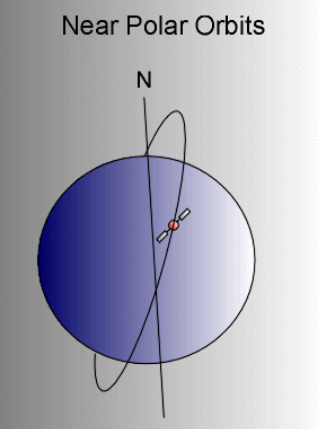
\includegraphics[width=0.3\textwidth]{img/near_polar_orbit.png}
	\caption{Direct solar radiation in near polar orbit}
	\label{fig:near_polar_orbit}
\end{figure}


\begin{table}[h!]
	\centering
	\begin{tabular}{c c c c c}
		\hline
		\textbf{Component} & \textbf{Optical property} & $\alpha$ & $\epsilon$ & $\frac{\alpha}{\epsilon}$ \\ \hline
		Structure & Black anodize & 0.88 & 0.88 & 1.0 \\ \hline
		Solar cell & ITO-GaAs & 0.92 & 0.85 & 1.1 \\ \hline
	\end{tabular}
	\caption{State-Summary of thermo-optical properties}
	\label{tab:passive_thermal}
\end{table}

In contrast, the worst cold condition corresponds to the case in which the satellite
is operated at the emergency mode
The danger of freezing is very small during regular operation. The experiences
from previous missions show that the heat of electrical components generated
during operation, as well as the radiation from the earth and the sun, are sufficient
to remain operational in the LEO. In addition, the entire orbit can never be in
eclipse, so there will always be a warm-up cycle during one period around the earth \cite{Hindawi}.

The heat radiation of the satellite without Solar Panels can be calculated as follows:

\begin{equation}
	P_{emit} = -A \epsilon \sigma T^4
\end{equation}

, where the Boltzmann constant, $\sigma = 5.67\cdot 10^{-8} W m^{-2} K^{-4}$

\begin{table}[h!]
	\centering
	\begin{tabular}{c c c c c}
		\hline
		\textbf{Radiation to space} & \textbf{Emissivity} & Area ($m^2$) & T(K) & Energy (W) \\ \hline
		Structure (Aluminum) & 0.77 & 0.1738 & 298.15 & -60.0 \\ \hline
	\end{tabular}
	\caption{State-Summary of thermo-optical properties}
	\label{tab:passive_thermal}
\end{table}

The direct solar flux can be calculated as shown:


\begin{equation}
	P_{sun} = A \alpha S \cos{\phi}
\end{equation}

, with $\cos{\phi} \approx 1$ and $\alpha \approx 1$

The albedo of earth’s atmosphere can be calculated as follows:

\begin{equation}
	P_{albedo} = A \alpha_{albedo} S 0.35 \cos{\phi} \left(\frac{R_{Earth}}{R_{sat}} \right)^2
\end{equation}

, with $\cos{\phi} \approx 1$ and $\alpha_{albedo} \approx 1$

The infrared radiation of the earth is calculated as follows:

\begin{equation}
	P_{albedo} = A_{Earth} \epsilon_{Earth} 236 \left(\frac{R_{Earth}}{R_{sat}} \right)^2 \cos{\phi}
\end{equation}

, with $\cos{\phi} \approx 1$, $\epsilon_{Earth} \approx 1$, $A_0 = 0.1562m^2$ and $A_{large} = 0.03m^2$

\begin{table}[h!]
	\centering
	\begin{tabular}{c c c c c c}
		\hline
		& \textbf{Hot Case} & \textbf{Area max} & $R_{Earth}$ & $R_{sat}$ & Energy \\
		& $W/m^2$ & $m^2$ & km & km & W \\ \hline
		Solar radiation & 1365 - 1373 & 0.03 & & & 41.2 \\ \hline
		Albedo & 409.5 - 411.9 & 0.06 & 6371 & 6971 & 20.6 \\ \hline
		Earth radiation & 236 & 0.06 & 6371 & 6971 & 11.8 \\ \hline
		Power consumption & & & & & 12.5 \\ \hline
		All & & & & & 86.2 \\ \hline
	\end{tabular}
	\caption{List of incoming heat sources}
	\label{tab:incomeing_heat}
\end{table}

\begin{table}[h!]
	\centering
	\begin{tabular}{c c c c c}
		\hline
		\textbf{Radiation to space} & \textbf{Emissivity} & Area ($m^2$) & T(K) & Energy (W) \\ \hline
		Structure (Aluminum) & 0.77 & 0.1738 & 298.15 & -60.0 \\ \hline
		Louvers & & & & -14.0 \\ \hline
		Solar panels (Si) & 0.85 & 0.05184 & & -10.0 \\ \hline
		All & & & & -84.0 \\ \hline
	\end{tabular}
	\caption{List of outcoming heat sources}
	\label{tab:heat_outcome}
\end{table}

This conservative calculation shows that a thermal equilibrium can occur.
The temperature fluctuations will be small because the dynamic louvers serve
as a buffer. The heat radiation of the solar panels has been estimated at -10W.
The heat radiation by albedo and earth radiation are also conservative and will
therefore be smaller in reality. The danger of overheating is averted by the
louvers.

Taking into account that due to passive attitude stabilization method using a
permanent magnet combined with hysteresis dampers the satellite is doing two
rotations per orbit. This provides the advantage of thermal stabilization of the
satellite because the angle between the CubeSat and the solar flux vector is
continuously changing \cite{wiki_thermal}.

Finally next table \ref{tab:temp_limit}, shows the temperature limits for every device in the subsystems
of the S/C:

\begin{table}[]
	\begin{tabular}{lllll}
		\hline
		& \multicolumn{2}{l}{Operating Temperatures} & \multicolumn{2}{l}{Surviving temperatures} \\
		Components                                 & Tmin ($^\circ$)& Tmax ($^\circ$)& Tmin ($^\circ$)& Tmax ($^\circ$)  \\ \hline
		ISIS TXS High Data rate S-band transmitter & -10                  & 55                  & -40                  & 60                  \\
		Helios deployable antenna                  & -15                  & 50                  & -60                  & 60                  \\
		Deployable turnstile antenna system        & -10                  & 50                  & -20                  & 60                  \\
		Solar Panels                               & -40                  & 125                 & -60                  & 140                 \\
		Battery                                    & -5                   & 45                  & -15                  & 60                  \\
		Structures                                 & -40                  & 80                  & -50                  & 100                 \\
		NanoMind CPU                               & -30                  & 85                  & -45                  & 95 \\ \hline
	\end{tabular}
	\caption{Temperature limits for all devices in the spacecraft}
	\label{tab:temp_limit}
\end{table}
